%iffalse
\documentclass[journal]{IEEEtran}
\usepackage[a5paper, margin=10mm]{geometry}
%\usepackage{lmodern} % Ensure lmodern is loaded for pdflatex
\usepackage{tfrupee} % Include tfrupee package


\setlength{\headheight}{1cm} % Set the height of the header box
\setlength{\headsep}{0mm}     % Set the distance between the header box and the top of the text


%\usepackage[a5paper, top=10mm, bottom=10mm, left=10mm, right=10mm]{geometry}

%
\setlength{\intextsep}{10pt} % Space between text and floats

\makeindex


\usepackage{cite}
\usepackage{amsmath,amssymb,amsfonts,amsthm}
\usepackage{algorithmic}
\usepackage{graphicx}
\usepackage{textcomp}
\usepackage{xcolor}
\usepackage{txfonts}
\usepackage{listings}
\usepackage{enumitem}
\usepackage{mathtools}
\usepackage{gensymb}
\usepackage{comment}
\usepackage[breaklinks=true]{hyperref}
\usepackage{tkz-euclide} 
\usepackage{listings}
\usepackage{multicol}
\usepackage{xparse}
\usepackage{gvv}
%\def\inputGnumericTable{}                                 
\usepackage[latin1]{inputenc}                                
\usepackage{color}                                            
\usepackage{array}                                            
\usepackage{longtable}                                       
\usepackage{calc}                                             
\usepackage{multirow}                                         
\usepackage{hhline}                                           
\usepackage{ifthen}                                               
\usepackage{lscape}
\usepackage{tabularx}
\usepackage{array}
\usepackage{float}


\newtheorem{theorem}{Theorem}[section]
\newtheorem{problem}{Problem}
\newtheorem{proposition}{Proposition}[section]
\newtheorem{lemma}{Lemma}[section]
\newtheorem{corollary}[theorem]{Corollary}
\newtheorem{example}{Example}[section]
\newtheorem{definition}[problem]{Definition}
\newcommand{\BEQA}{\begin{eqnarray}}
\newcommand{\EEQA}{\end{eqnarray}}

\theoremstyle{remark}


\begin{document}
\bibliographystyle{IEEEtran}
\onecolumn

\title{GATE 2007 AE 18-24}
\author{ee24btech11015 - Dhawal}
\maketitle

\renewcommand{\thefigure}{\theenumi}
\renewcommand{\thetable}{\theenumi}

\begin{enumerate}[start=18]
	\item Across a normal shock
\begin{enumerate}
\item both total temperature and total pressure decrease 
\item both total temperature and total pressure remain constant 
\item total pressure remains constant but total temperature decreases 
\item total temperature remains constant but total pressure decreases
\end{enumerate}

\item  The Joukowskii airfoil is studied in aerodynamics because
\begin{enumerate}
\item it is used in many aircraft
\item it is easily transformed into a circle, mathematically
\item it has a simple geometry
\item it has the highest lift curve slope among all airfoils
\end{enumerate}

\item  One of the criteria for high-speed airplanes is that the critical Mach number should be as high as possible. Therefore, high-speed subsonic airplanes are usually designed with 
\begin{multicols}{2}
\begin{enumerate}
\item thick airfoils
\item thin airfoils
\item laminar flow airfoils
\item diamond airfoils
\end{enumerate}
\end{multicols}

\item  Two identical earth satellites $A$ and $B$ are in circular orbits at altitudes $h_A$ and $h_B$ above the earth's surface respectively, with $h_A > h_B$. If $E$ denotes the total mechanical energy, $T$ the kinetic energy and $V$ the gravitational potential energy of a satellite, then:
\begin{multicols}{2}
\begin{enumerate}
\item $E_A > E_B \text{ and } V_A < V_B$
\item $E_A > E_B \text{ and } T_A > T_B$
\item $E_A < E_B \text{ and } T_A > T_B$
\item $E_A > E_B \text{ and } T_A < T_B$
\end{enumerate}
\end{multicols}

\item  Let $P$ and $Q$ be two square matrices of same size. Consider the following statements
\begin{align}
    PQ=0 \text{ implies } P=0 \text{ or } Q=0 \text{ or both }
\end{align}
\begin{align}
    PQ=I^2 \text{ implies } P=Q^{-1}
\end{align}
\begin{align}
    {\brak{P+Q}}^2 =P^2+2PQ+Q^2
\end{align}
\begin{align}
     {\brak{P-Q}}^2 =P^2-2PQ+Q^2
\end{align}
where $I$ is the identity matrix. Which of the following statements is correct?
\begin{multicols}{2}
\begin{enumerate}
\item 1, 2 and 3 are false, but 4 is true
\item 1, 2 and 4 are false, but 3 is true
\item 2, 3 and 4 are false, but 1 is true 
\item 1, 3 and 4 are false, but 2 is true
\end{enumerate}
\end{multicols}

\item   A 1 kg mass attached to a spring elongates it by 16 mm. The mass is then pulled from its equilibrium position by 10 mm and released from rest. Assuming the acceleration due to gravity of $9.81 \, \text{m/s}^2$, the response of the mass in mm is given by
\begin{multicols}{2}
\begin{enumerate}
\item $x=10 \sin\brak{24.76t}$
\item $x=10 \cos\brak{24.76t}$
\item $x=\sin\brak{16t}$
\item $x=10\cos\brak{16t}$
\end{enumerate}
\end{multicols}

\item  The earth's radius is $6.37 \times 10^6$ m and the acceleration due to gravity on its surface is $9.81 \, \text{m/s}^2$. A satellite is in a circular orbit at a height of $6.30 \times 10^5$ m above the earth's surface. The minimum additional speed it needs to escape from the earth's gravitational field is
\begin{multicols}{2}
\begin{enumerate}
\item $3.66 \times 10^3 \, \text{m/s}$
\item $3.12 \times 10^3 \, \text{m/s}$
\item $3.27 \times 10^3 \, \text{m/s}$
\item $3.43 \times 10^3 \, \text{m/s}$
\end{enumerate}
\end{multicols}

\item  Shown in the figure below is a model of an Euler-Bernoulli beam made up of two materials subjected to pure bending moment $M$. The Young's modulus of material A and B are $E_A$ and $E_B$, respectively. The sectional moment of area, about the neutral axis, of the cross-sectional areas made of materials A and B, are $I_A$ and $I_B$, respectively. The radius of curvature $\rho$ of the flexural deflection of this composite beam to the bending moment $M$ is then:
\begin{center}
    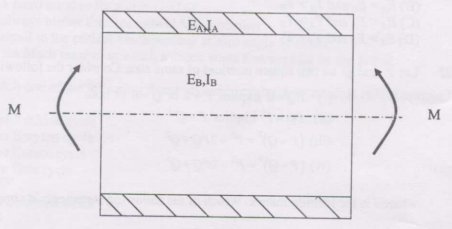
\includegraphics[width=0.6\textwidth]{beam.png}
\end{center}


\begin{multicols}{4}
\begin{enumerate}
\item $\rho = \frac{E_A I_A + E_B I_B}{M}$
\item $\rho = \frac{E_B I_B + E_A I_A}{M}$
\item $\rho = \frac{M}{E_A I_A + E_B I_B}$
\item $\rho = \frac{\brak{E_A + E_B}\brak{I_A + I_B}}{M}$
\end{enumerate}
\end{multicols}

\item  Two pipes of constant sections but different diameters carry water at the same volume flow rate. The Reynolds number, based on the pipe diameter, is:
\begin{multicols}{2}
\begin{enumerate}
\item the same in both pipes
\item is larger in the narrower pipe
\item is smaller in the narrower pipe
\item depends on the material of the pipes
\end{enumerate}
\end{multicols}

\item  Two airfoils of the same family are operating at the same angle of attack. The dimensions of one airfoil are twice as large as the other one. The ratio of the minimum pressure coefficient of the larger airfoil to the minimum pressure coefficient of the smaller airfoil is: 
\begin{multicols}{4}
\begin{enumerate}
\item 4
\item 2
\item 1
\item 0.5
\end{enumerate}
\end{multicols}

\item  Wing A has a constant chord $c$ and span $b$. Wing B is identical but has a span $4b$. When both wings are operating at the same geometric angle of attack at subsonic speed, then:
\begin{enumerate}
\item wings A and B produce the same lift coefficient
\item wing A produces a smaller lift coefficient than wing B
\item wing A produces a greater lift coefficient than wing B
\item the freestream Mach number decides which wing produces the greater lift coefficient.
\end{enumerate}

\item  A spring-mass-damper system is excited by a force $F_0 \sin \omega t$. The amplitude at resonance is measured to be 1 cm. At half the resonant frequency, the amplitude is 0.5 cm. The damping ratio of the system is:
\begin{multicols}{4}
\begin{enumerate}
\item 0.1026
\item 0.3242
\item 0.7211
\item 0.1936
\end{enumerate}
\end{multicols}

\item  The eigenvalues of the matrix, 
$ A = \myvec{2 & 1 \\0 & 3}$
are:
\begin{multicols}{4}
\begin{enumerate}
\item 1 and 2
\item 1 and 3
\item 2 and 3
\item 2 and 4
\end{enumerate}
\end{multicols}

\item  The eigenvalues of the matrix $A^{-1}$, where 
$ A = \myvec{2 & 1 \\0 & 3}$
are:
\begin{multicols}{4}
\begin{enumerate}
\item $1 \text{ and } \frac{1}{2}$
\item $1 \text{ and } \frac{1}{3}$
\item $2 \text{ and } 3$
\item $\frac{1}{2} \text{ and } \frac{1}{3}$

\end{enumerate}
\end{multicols}

\item  The radius of the earth is $6.37 \times 10^6 \, \text{m}$ and the acceleration due to gravity at its surface is $9.81 \, \text{m/s}^2$. A satellite is in circular orbit at a height of $35.9 \times 10^6 \, \text{m}$ above the earth's surface. This orbit is inclined at $10.5^\circ$ to the equator. The velocity change needed to make the orbit equatorial is:
\begin{enumerate}
\item 561 m/s at $84.75\degree$ to the initial direction
\item 561 m/s at $95.25\degree$ to the initial direction
\item 281 m/s at $84.75\degree$ to the initial direction
\item 281 m/s at $95.25\degree$ to the initial direction
\end{enumerate}

\item  A piston-prop airplane having propeller efficiency, $\eta_p = 0.8$, and weighing $73108 \, \text{N}$ could achieve maximum climb rate of $15 \, \text{m/s}$ at flight speed of $50 \, \text{m/s}$. The excess Brake Power (BP) at the above flight condition will be:
\begin{multicols}{4}
\begin{enumerate}
\item 1700 kW
\item 2100 kW
\item 1371 kW
\item 6125 kW
\end{enumerate}
\end{multicols}
\item  An airplane model with a symmetric airfoil was tested in a wind tunnel. $C_{m}$ (moment coefficient, at angle of attack, $\alpha = 0$) was estimated to be 0.08 and 0 respectively for elevator settings ($\delta_e$) of $5 \degree$ up and $5 \degree$ down. The estimated value of the elevator control power $\left( \frac{\partial C_m}{\partial \delta_e} \right)$ of the model will be:
\begin{multicols}{4}
\begin{enumerate}
\item $0.07 / \degree$
\item $-1.065 / \degree$
\item $-0.008 / \degree$
\item $-0.762 / \degree$
\end{enumerate}
\end{multicols}



\end{enumerate}


\end{document}

